
\documentclass[letterpaper,12pt,titlepage,oneside,final]{book}
\usepackage[pdftex]{graphicx} % For including graphics N.B. pdftex graphics driver 
\usepackage{amsmath,amssymb,amstext, amsthm} % Lots of math symbols and environments

%----------------------------------------------------------------------------------------
% Mods
%----------------------------------------------------------------------------------------
\usepackage[capitalise]{cleveref}
\usepackage{nameref}

\usepackage{csquotes}
\MakeOuterQuote{"}

\usepackage{floatpag}
\floatpagestyle{empty}

\usepackage{caption}
\captionsetup{font=scriptsize}

\usepackage{dsfont}

\newtheorem{theorem}{Theorem}[section]
\newtheorem{lemma}[theorem]{Lemma}
\newtheorem{proposition}[theorem]{Proposition}
\newtheorem{claim}[theorem]{Claim}
\newtheorem{corollary}[theorem]{Corollary}
\newtheorem{definition}[theorem]{Definition}
\newtheorem{remark}[theorem]{Remark}
\newtheorem{example}[theorem]{Example}
\newtheorem{problem}[theorem]{Problem}
\newtheorem{condition}[theorem]{Condition}
\renewenvironment{proof}{{\bf Proof:}}{\hfill\rule{2mm}{2mm}}
\newenvironment{outline}{{\bf Outline:}}

\newcommand\E{\mathbb{E}}
\newcommand{\abs}[1]{\lvert#1\rvert}
\newcommand{\norm}[1]{\lVert#1\rVert}
\newcommand{\bigabs}[1]{\bigl\lvert#1\bigr\rvert}
\newcommand{\bignorm}[1]{\bigl\lVert#1\bigr\rVert}
\newcommand{\term}[1]{{\textit{\textbf{#1}}}}
\newcommand{\bd}[1]{{\mathbf{\textbf{#1}}}}
\newcommand{\marg}[1]{\marginpar{\tiny #1}}
\newcommand{\MU}{\boldsymbol\mu}
\newcommand{\LAMBDA}{\boldsymbol\lambda}
\newcommand{\inv}{\leftarrow}
\newcommand{\var}{\text{VaR}}
\newcommand{\overbar}[1]{\mkern 1.5mu\overline{\mkern-1.5mu#1\mkern-1.5mu}\mkern 1.5mu}
\newcommand*\red{\color{red}}

\interfootnotelinepenalty=10000
%----------------------------------------------------------------------------------------
%----------------------------------------------------------------------------------------


\begin{document}
	
	\begin{figure}
		\centering
		\begin{minipage}{0.45\textwidth}
			\centering
			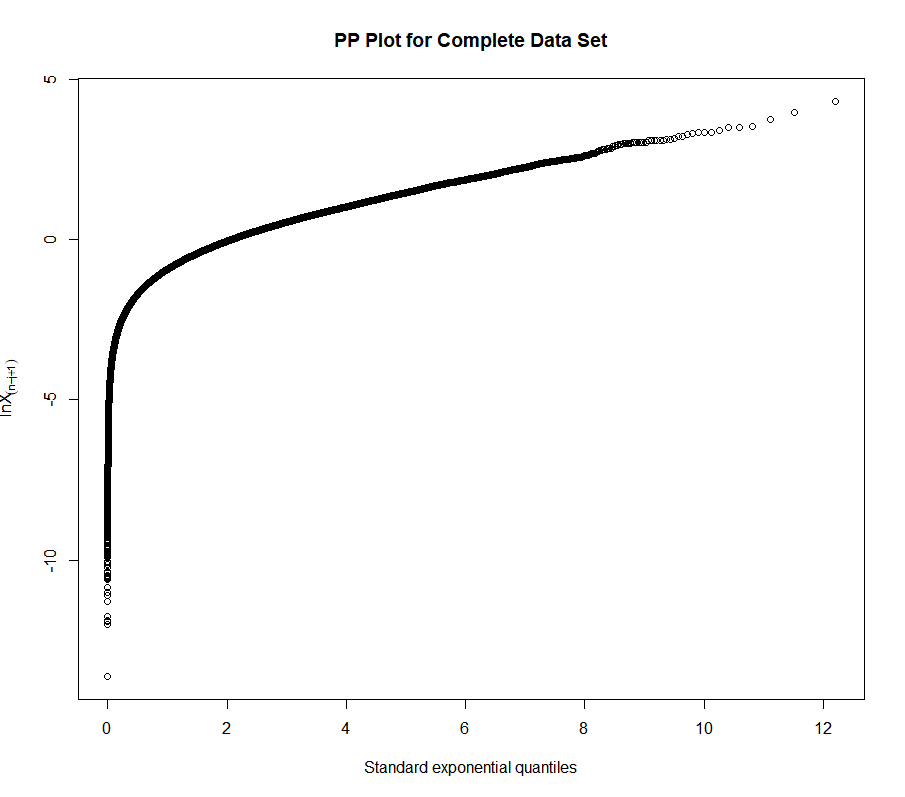
\includegraphics[width=0.9\textwidth]{ParWhole}
			\caption{PP Plot for Entire Pareto Set}
			\label{fig: ParWhole}
		\end{minipage}\hfill
		\begin{minipage}{0.45\textwidth}
			\centering
			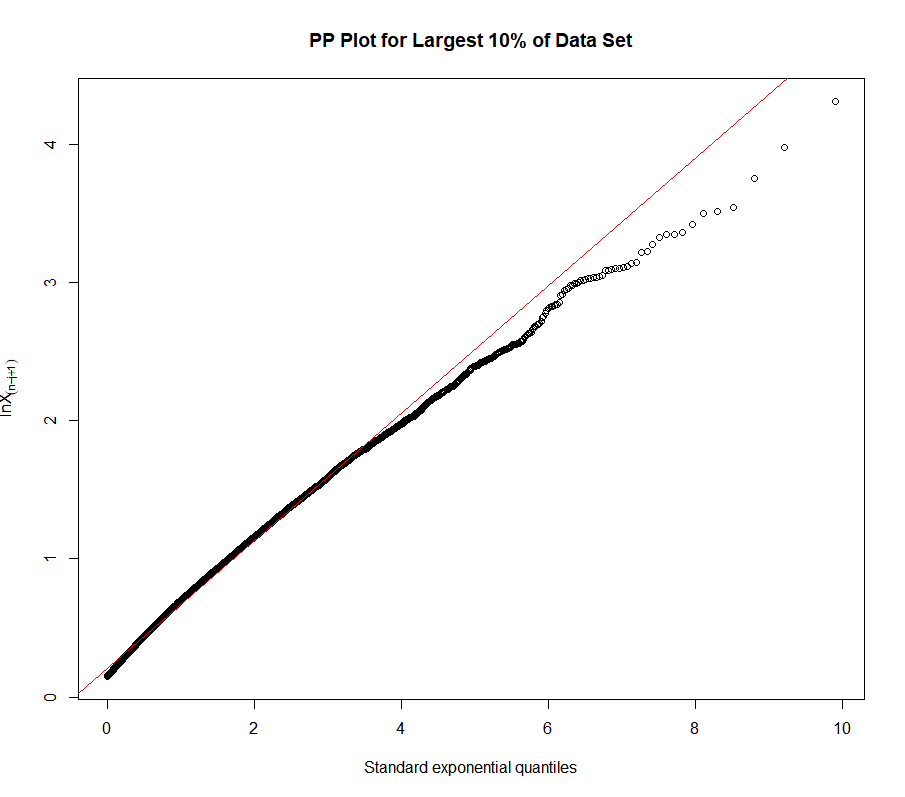
\includegraphics[width=0.9\textwidth]{Pare10}
			\caption{PP Plot for Largest 10\% of Pareto Set}
			\label{fig: Pare10}
		\end{minipage}
	\end{figure}

Above are the Zipf plots for 200000 randomly generated realizations from a Pareto Random Variable with parameter 3. We can see the the typical behaviour of such a plot for the entire data set as well as the largest 10\% of the realizations. The red line is a fitted line using linear regression.

\vspace{5mm}

\noindent\begin{minipage}{\textwidth}
	\begin{minipage}{0.45\textwidth}
		\centering
		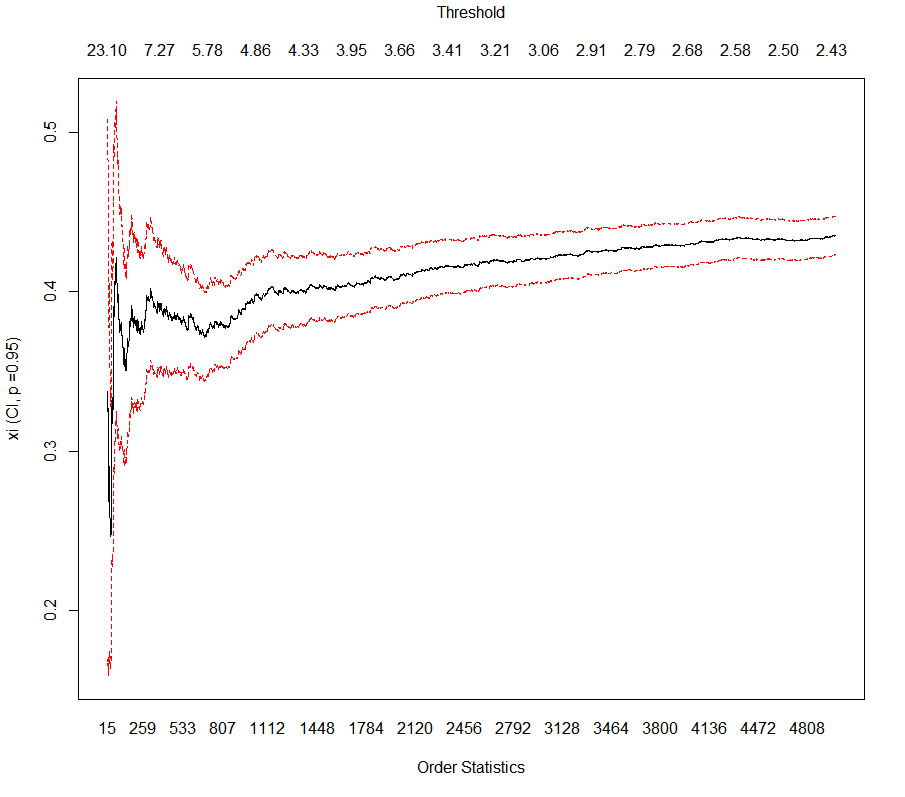
\includegraphics[width=0.9\textwidth]{ParHill}
		\captionof{figure}{Hill Plot of Largest 5000 Order statistics}
	\end{minipage}
	\hfill
	\begin{minipage}[b]{0.45\textwidth}
		\centering
	\captionof{table}{The Hill estimates for Pareto with parameter 3. Standard errors are in parenthesis.} 
	\label{tab: Pareto Hill} 
	\scriptsize
	\makebox[0pt][c]{\parbox{\textwidth}{%
			\begin{minipage}[b]{\hsize}\centering
				\begin{tabular}{@{\extracolsep{5pt}} cccc}
					\\[-1.8ex]\hline 
					\hline \\[-1.8ex]
					&\multicolumn{3}{c}{Right Tail}\\ 
					k				&   			  $2000$&				  $3000$&		$4000$\\ 
					\hline \\[-1.8ex] 
					$ X_{i}$ & 		$0.4081(0.009)$&		$0.4211(0.007)$&		$0.4300(0.006)$\\ 
				\end{tabular} 
			\end{minipage}%
	}}
	\end{minipage}
\end{minipage}

Hence, we can say that $\xi \approx 0.42$, then tail density is  $1 - F(x) \to \mathcal{L}(x) ^{-2.38}$ as $x$ get sufficiently large. This is close enough to the original Pareto Parameter.

Simliarly, if we have another 200000 realizations with pareto parameter 2, we have the following Hill Plot and Estimators.

\noindent\begin{minipage}{\textwidth}
	\begin{minipage}{0.45\textwidth}
		\centering
		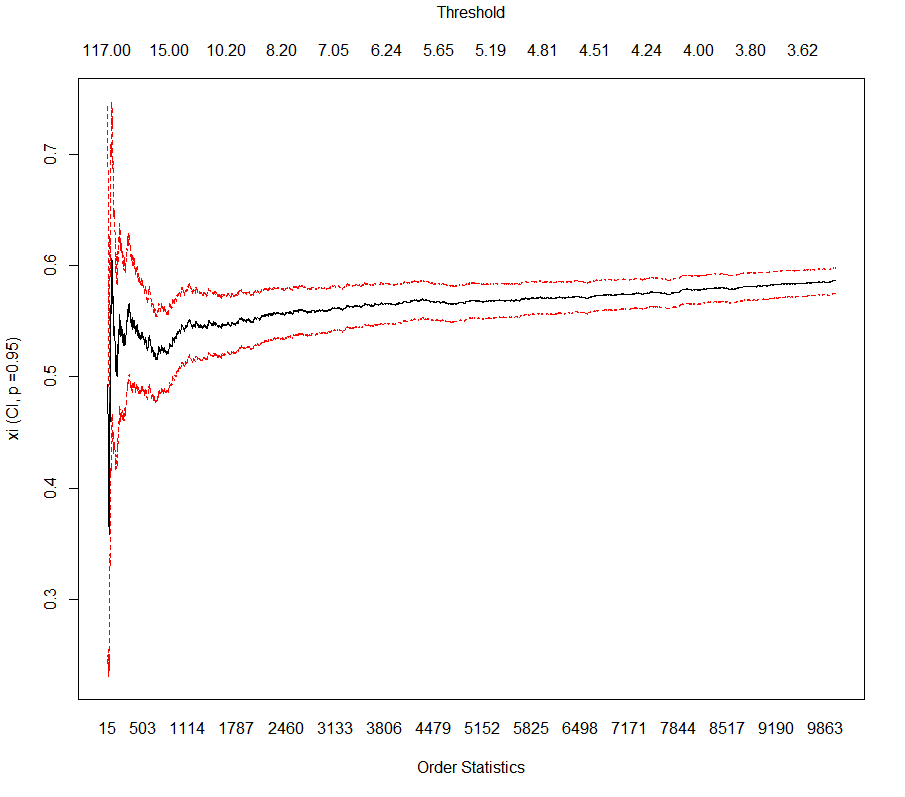
\includegraphics[width=0.9\textwidth]{ParHill2}
		\captionof{figure}{Hill Plot of Largest 5000 Order statistics}
	\end{minipage}
	\hfill
	\begin{minipage}[b]{0.45\textwidth}
		\centering
		\captionof{table}{The Hill estimates for Pareto with parameter 3. Standard errors are in parenthesis.} 
		\label{tab: Pareto Hill2} 
		\scriptsize
		\makebox[0pt][c]{\parbox{\textwidth}{%
				\begin{minipage}[b]{\hsize}\centering
					\begin{tabular}{@{\extracolsep{5pt}} cccc}
						\\[-1.8ex]\hline 
						\hline \\[-1.8ex]
						&\multicolumn{3}{c}{Right Tail}\\ 
						k				&   			  $2000$&				  $3000$&		$4000$\\ 
						\hline \\[-1.8ex] 
						$ X_{i}$ & 		$0.5495(0.012)$&		$0.5597(0.0102)$&		$0.5659(0.0089)$\\ 
					\end{tabular} 
				\end{minipage}%
		}}
	\end{minipage}
\end{minipage}

Hence, we can say that $\xi \approx 0.55$, then tail density is  $1 - F(x) \to \mathcal{L}(x) ^{-1.82}$ as $x$ get sufficiently large. This is close enough to the Pareto Parameter 2.


If you take instead 200000 realizations from a standard normal distribution, we have the following Zipf plots
	
		\begin{figure}
		\centering
		\begin{minipage}{0.45\textwidth}
			\centering
			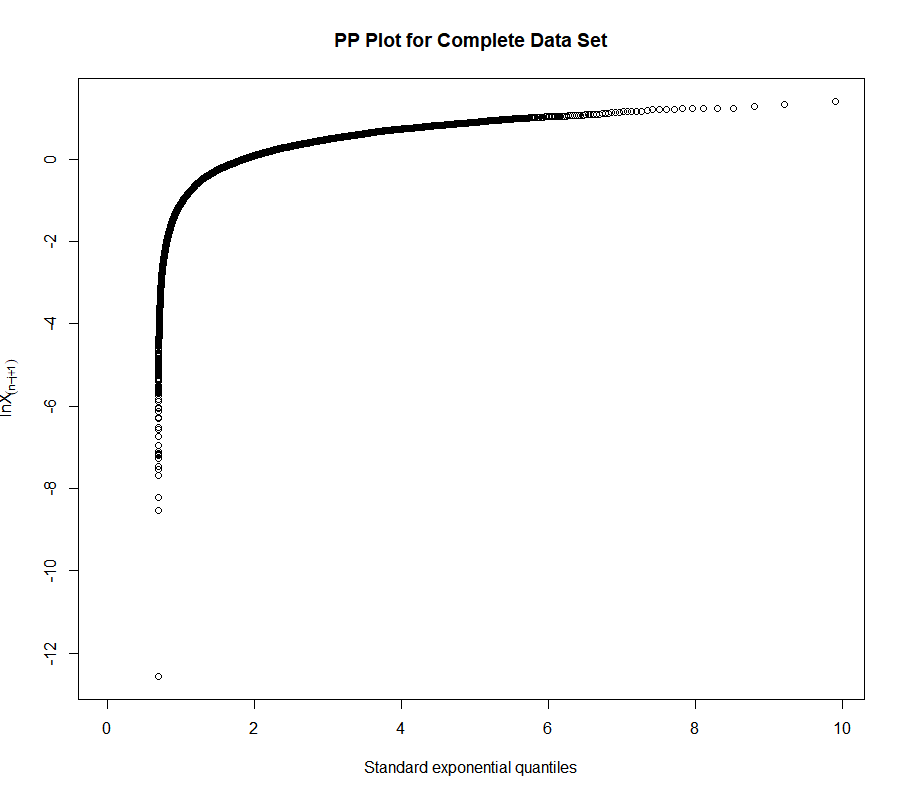
\includegraphics[width=0.9\textwidth]{NormWhole}
			\caption{PP Plot for Entire Normal Set}
			\label{fig: NormWhole}
		\end{minipage}\hfill
		\begin{minipage}{0.45\textwidth}
			\centering
			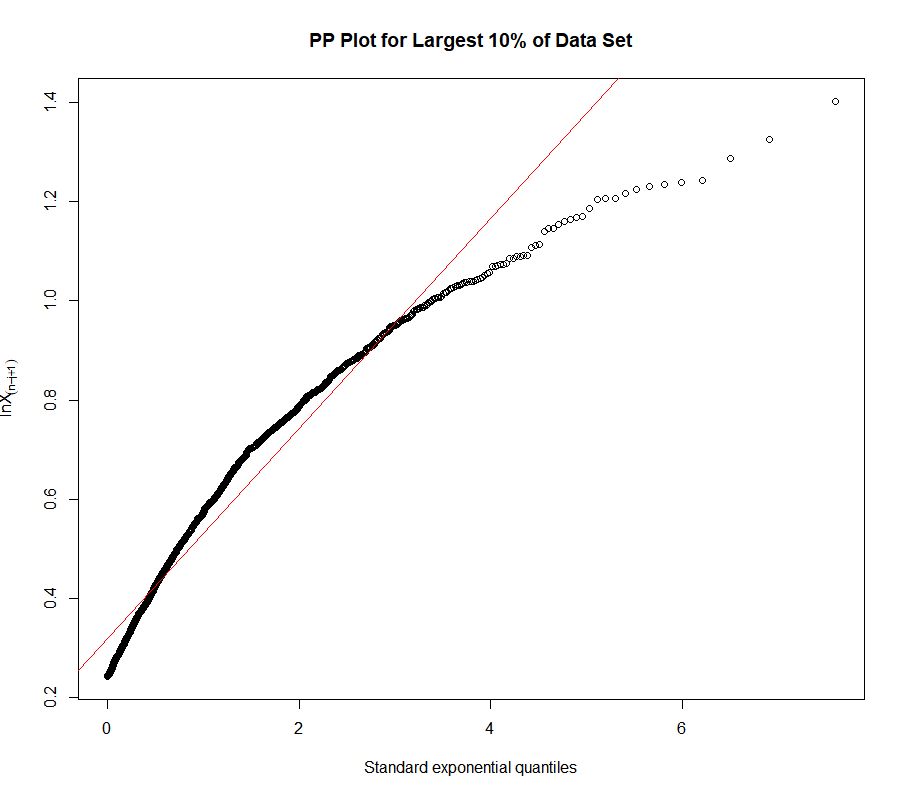
\includegraphics[width=0.9\textwidth]{Norm10}
			\caption{PP Plot for Largest 10\% of Normal Set}
			\label{fig: Norm10}
		\end{minipage}
	\end{figure}

 \pagebreak

In constrast to the Pareto, we see that the largest 10\% of the data set shows non-linearity and bows away from the fitted least squares line, suggesting thinner tails. 

Below is the Hill Plot for the Largest 5000 order statistics. We can see even in such a small subset, there is no region of stability, making it much more difficult to estimate $\xi$.

\noindent\begin{minipage}{\textwidth}
	\begin{minipage}{0.45\textwidth}
		\centering
		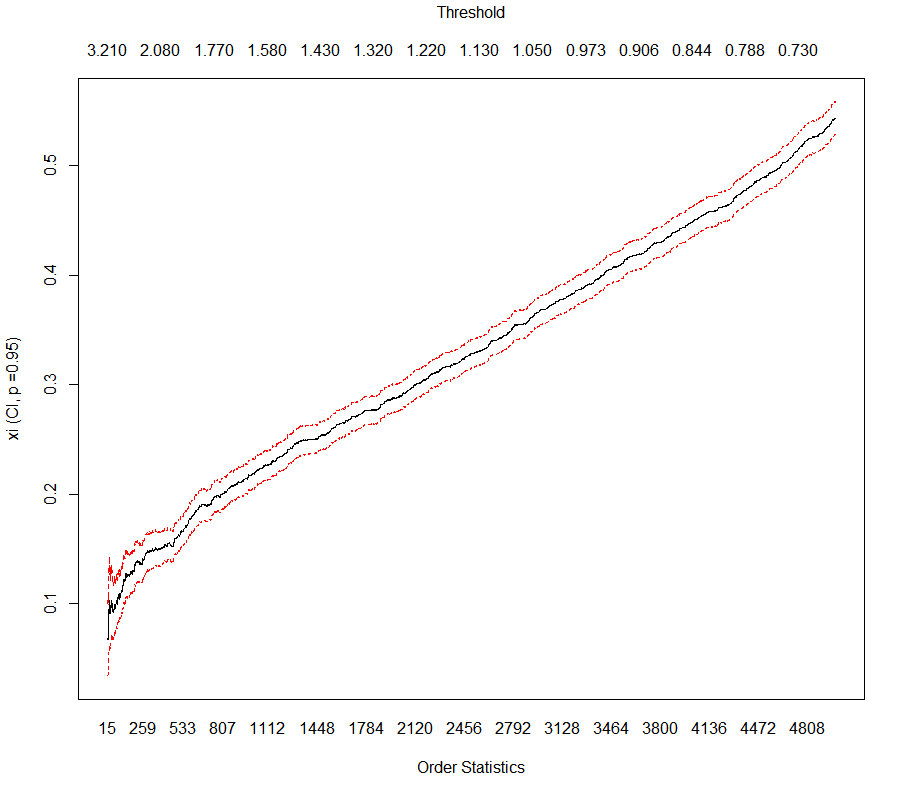
\includegraphics[width=0.9\textwidth]{NormHill}
		\captionof{figure}{Hill Plot of Largest 5000 Order statistics}
	\end{minipage}
	\hfill
	\begin{minipage}[b]{0.45\textwidth}
		\centering
		\captionof{table}{The Hill estimates for Standard Normal. Standard errors are in parenthesis.} 
		\label{tab: NormHill} 
		\scriptsize
		\makebox[0pt][c]{\parbox{\textwidth}{%
				\begin{minipage}[b]{\hsize}\centering
					\begin{tabular}{@{\extracolsep{5pt}} cccc}
						\\[-1.8ex]\hline 
						\hline \\[-1.8ex]
						&\multicolumn{3}{c}{Right Tail}\\ 
						k				&   			  $2000$&				  $3000$&		$4000$\\ 
						\hline \\[-1.8ex] 
						$ Y_{i}$ & 		$0.2882(0.006)$&		$0.3687(0.006)$&		$0.4478(0.007)$\\ 
					\end{tabular} 
				\end{minipage}%
		}}
	\end{minipage}
\end{minipage}


In general, there is no hard a fast rule for choosing k. We use heurestic rules to find regions where the Hill Plot becomes stable. That is, find a region in the hill plot where the variance subsides seems to subside. This is referred to as the "Eye-Ball technique"\cite{danielsson2016tail}.
	



\begin{thebibliography}{9}
	\bibitem{danielsson2016tail} 
	Danielsson, Jon and Ergun, Lerby Murat and de Haan, Laurens and de Vries, Casper G. 
	\textit{Tail index estimation: Quantile driven threshold selection}. 
	Available at SSRN 2717478, 2016.
\end{thebibliography}


	
	
\end{document}
